\documentclass[border=0.110cm]{standalone}
\usepackage{tikz}
\usetikzlibrary{arrows.meta}
\definecolor{sqGray}{HTML}{B5B5B5}
\begin{document}
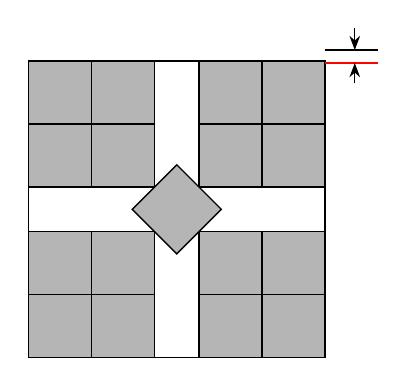
\begin{tikzpicture}[x=0.800cm,y=0.800cm]
  \filldraw[fill=sqGray,draw=black,line width=0.5pt] (0.00000,0.00000) rectangle (1.00000,1.00000);
  \filldraw[fill=sqGray,draw=black,line width=0.5pt] (0.00000,1.00000) rectangle (1.00000,2.00000);
  \filldraw[fill=sqGray,draw=black,line width=0.5pt] (1.00000,0.00000) rectangle (2.00000,1.00000);
  \filldraw[fill=sqGray,draw=black,line width=0.5pt] (1.00000,1.00000) rectangle (2.00000,2.00000);
  \filldraw[fill=sqGray,draw=black,line width=0.5pt] (0.00000,2.70711) rectangle (1.00000,3.70711);
  \filldraw[fill=sqGray,draw=black,line width=0.5pt] (0.00000,3.70711) rectangle (1.00000,4.70711);
  \filldraw[fill=sqGray,draw=black,line width=0.5pt] (1.00000,2.70711) rectangle (2.00000,3.70711);
  \filldraw[fill=sqGray,draw=black,line width=0.5pt] (1.00000,3.70711) rectangle (2.00000,4.70711);
  \filldraw[fill=sqGray,draw=black,line width=0.5pt] (2.70711,0.00000) rectangle (3.70711,1.00000);
  \filldraw[fill=sqGray,draw=black,line width=0.5pt] (2.70711,1.00000) rectangle (3.70711,2.00000);
  \filldraw[fill=sqGray,draw=black,line width=0.5pt] (3.70711,0.00000) rectangle (4.70711,1.00000);
  \filldraw[fill=sqGray,draw=black,line width=0.5pt] (3.70711,1.00000) rectangle (4.70711,2.00000);
  \filldraw[fill=sqGray,draw=black,line width=0.5pt] (2.70711,2.70711) rectangle (3.70711,3.70711);
  \filldraw[fill=sqGray,draw=black,line width=0.5pt] (2.70711,3.70711) rectangle (3.70711,4.70711);
  \filldraw[fill=sqGray,draw=black,line width=0.5pt] (3.70711,2.70711) rectangle (4.70711,3.70711);
  \filldraw[fill=sqGray,draw=black,line width=0.5pt] (3.70711,3.70711) rectangle (4.70711,4.70711);
  \filldraw[fill=sqGray,draw=black,line width=0.5pt,rotate around={45:(2.35355,2.35355)}]
    (1.85355,1.85355) rectangle (2.85355,2.85355);
  \draw[draw=black,line width=0.6pt] (0,0) rectangle (4.70711,4.70711);
  % две прямые размерные линии, раздвинутые для читаемости
  \draw[black,line width=0.4pt] (4.70711,4.88211) -- (5.55086,4.88211);
  \draw[red,line width=0.8pt] (4.70711,4.67553) -- (5.55086,4.67553);
  \draw[black,line width=0.45pt,-{Stealth[length=1.8mm]}] (5.17961,5.22711) -- (5.17961,4.88211);
  \draw[black,line width=0.45pt,-{Stealth[length=1.8mm]}] (5.17961,4.35553) -- (5.17961,4.67553);
\end{tikzpicture}
\end{document}
